\usetikzlibrary{arrows}
\begin{tikzpicture}[scale=0.7,transform shape]

 \node[anchor=south west,inner sep=0] at (0,0) {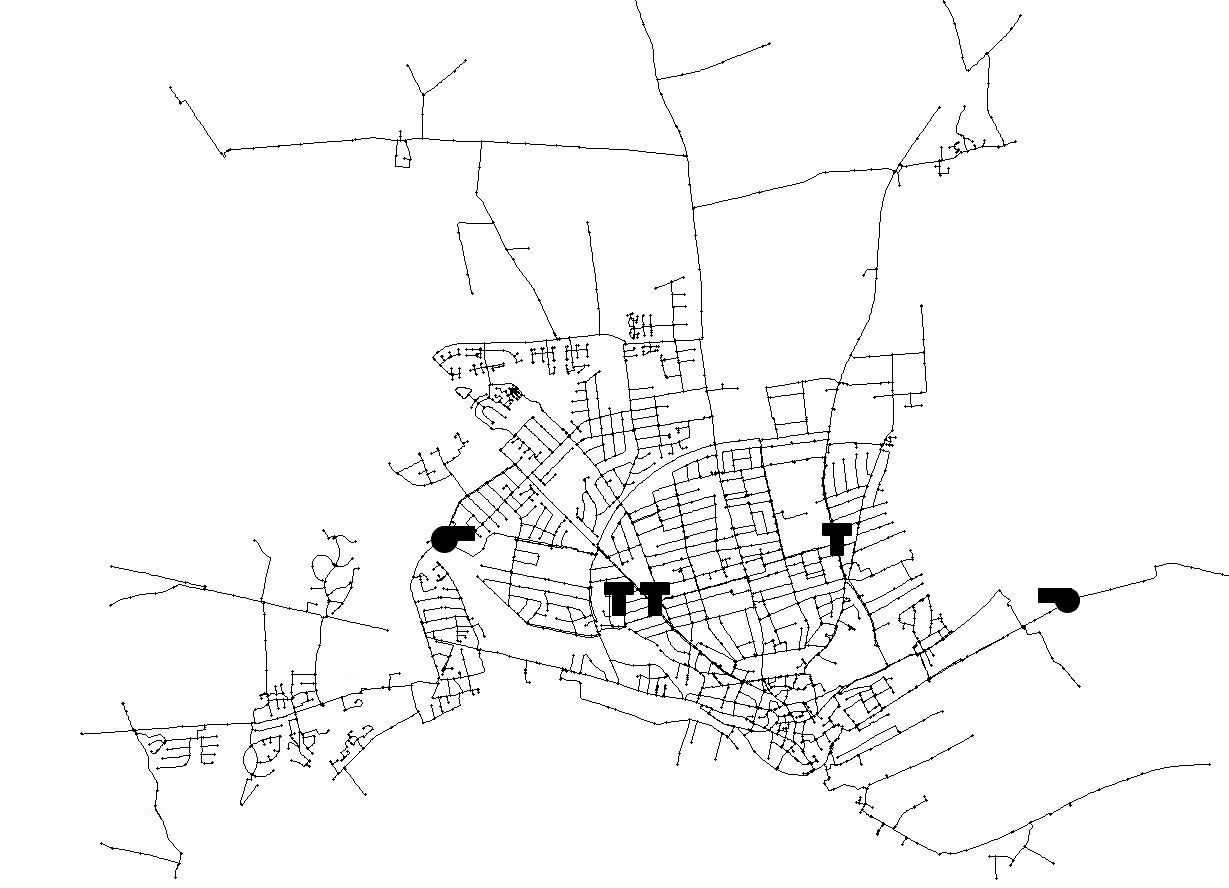
\includegraphics[width=\textwidth]{report/tikz/identification_map1}};
\node[black] at (11.4,4.75) {\footnotesize $\bm {\mathcal{W}_3}$};
\node[black] at (13.75,3.3) {\footnotesize $\bm {\mathcal{K}_2}$};
\node[black] at (4.7,4.65) {\footnotesize $\bm {\mathcal{K}_1}$};
\node[black] at (8.4,1) {\footnotesize $\bm {\mathcal{W}_2}$};
\node[black] at (6.8,1) {\footnotesize $\bm {\mathcal{W}_1}$};
\draw [-latex][thick](8.05,3.2) -- (8.4,1.35);
\draw [-latex][thick](7.55,3.2) -- (6.8,1.35);
\end{tikzpicture}
